\documentclass[twoside, a4paper, 12pt, spanish]{article}
\DeclareUnicodeCharacter{00A0}{\space}
\usepackage[spanish]{babel}
\usepackage{amsmath, amssymb}
\usepackage{siunitx}
\usepackage{graphicx}
\usepackage{float}
\usepackage{listings}
\usepackage{xcolor}
\usepackage{subcaption}
\usepackage[colorinlistoftodos]{todonotes} 
\usepackage{fancyhdr}
\pagestyle{fancy}
\usepackage{parskip}
\fancyhf{}             
\setlength{\headheight}{15.6pt}
% --- Definición de la paleta "Light High Contrast" ---
\definecolor{fondo_lhc}{RGB}{255, 255, 255}    % Fondo blanco puro
\definecolor{texto_lhc}{RGB}{0, 0, 0}          % Texto principal en negro puro
\definecolor{comentario_lhc}{RGB}{0, 100, 0}   % Comentarios en verde oscuro
\definecolor{palabra_lhc}{RGB}{0, 0, 255}      % Palabras clave en azul fuerte (def, import)
\definecolor{funcion_lhc}{RGB}{128, 0, 128}    % Funciones en púrpura intenso (np, plt)
\definecolor{numero_lhc}{RGB}{178, 34, 34}     % Números en rojo carmesí oscuro
% --- Configuración del entorno de código ---
\lstdefinestyle{tema_claro}{
    language=Python,
    backgroundcolor=\color{fondo_lhc},   
    basicstyle=\ttfamily\footnotesize\color{texto_lhc},
    commentstyle=\color{comentario_lhc},
    keywordstyle=\color{palabra_lhc}\bfseries,
    % Truco para colorear los dígitos de rojo oscuro
    literate=
        {0}{{\color{numero_lhc}0}}1
        {1}{{\color{numero_lhc}1}}1
        {2}{{\color{numero_lhc}2}}1
        {3}{{\color{numero_lhc}3}}1
        {4}{{\color{numero_lhc}4}}1
        {5}{{\color{numero_lhc}5}}1
        {6}{{\color{numero_lhc}6}}1
        {7}{{\color{numero_lhc}7}}1
        {8}{{\color{numero_lhc}8}}1
        {9}{{\color{numero_lhc}9}}1,
    % Forzamos las palabras específicas para que salgan en púrpura
    emph={v_verlet, np, plt, len, zeros, f, t_eval, x, v, a, dt, x0, v0, v_med, aceleracion_p1, factor, sqrt, linspace},
    emphstyle=\color{funcion_lhc},
    % Ajustes visuales generales
    breaklines=true,
    showspaces=false,
    showstringspaces=false,
    tabsize=4,
    % --- ESTRUCTURA (Números y línea vertical) ---
    numbers=left,                      % Activa los números a la izquierda
    numberstyle=\tiny\color{gray},     % Números de línea en gris (para no distraer del código)
    numbersep=15pt,                    % Separación entre los números y el código
    frame=l,                           % Crea únicamente la línea vertical a la izquierda
    framesep=10pt,                     % Distancia entre la línea vertical y el texto
    rulecolor=\color{texto_lhc},       % Línea vertical en negro puro
    xleftmargin=25pt,                  % Margen para acomodar los números
    framexleftmargin=25pt              % Expande el fondo (blanco) para cubrir los números
}
% Le decimos a LaTeX que use este estilo por defecto
\lstset{style=tema_claro}
% Encabezado con Logo
\lhead{\includegraphics[height=1.2cm]{Figures/Logos/Logo UNal.pdf}} 
\chead{\textbf{Universidad Nacional de Colombia}\\ \small Herramientas Computacionales}
\rhead{\thepage}
\renewcommand{\headrulewidth}{0.5pt}
\renewcommand{\footrulewidth}{0pt}
\renewcommand{\contentsname}{Contenidos}
% -----------------------
\raggedbottom
\usepackage{indentfirst}
\usepackage{verbatim}
\usepackage{textcomp}
\usepackage{gensymb}
\usepackage{relsize}
\usepackage{lipsum}
\usepackage{xparse}
\NewDocumentCommand{\myrule}{O{1pt} O{2pt} O{black}}{%
  \par\nobreak 
  \kern\the\prevdepth 
  \kern#2 
  {\color{#3}\hrule height #1 width\hsize} 
  \kern#2 
  \nointerlineskip 
}
\usepackage[section]{placeins}
\usepackage{booktabs}
\usepackage{colortbl}
   \newcommand{\myrowcolour}{\rowcolor[gray]{0.925}}
\usepackage[obeyspaces]{url}
\usepackage{etoolbox}
\usepackage[colorlinks, citecolor=black, urlcolor=blue, linkcolor=black, bookmarks=false, hypertexnames=true]{hyperref}
\usepackage{geometry}
\geometry{
	paper=a4paper,
	inner=3cm,
	outer=3cm,
	bindingoffset=.5cm,
	top=2.5cm, 
	bottom=2cm,
	headsep=1cm 
}

%_________________________________________________________%
\begin{document}
\begin{titlepage}
\begin{center}
\vspace*{3cm}
\textbf{\LARGE Universidad Nacional de Colombia}\\[0.5cm] 
\textbf{\Large Facultad de Ciencias}\\
\vspace{20pt}
\textbf{\large Departamento de Física}\\[0.2cm]
\vspace{20pt}
    \includegraphics[width=0.4\textwidth]{Figures/Logos/Escudo UNal.png}
\par
\vspace{20pt}
\textbf{\Large Herramientas Computacionales}\\
\vspace{15pt}
\myrule[1pt][7pt]
\textbf{\LARGE  Proyecto Intermedio}\\
\vspace{15pt}
\textbf{\large Simulación de guerra entre guerrillas}\\
\myrule[1pt][7pt]
\vspace{25pt}
\begin{minipage}{0.45\textwidth}
        \begin{flushleft} \large
            \textbf{Autores:}\\
            Sara Alba Mogollón\\
            Kéyner Alexander Avendaño\\
            Daniel Pérez Serna\\
        \end{flushleft}
    \end{minipage}
    \begin{minipage}{0.45\textwidth}
        \begin{flushright} \large
            \textbf{Profesor:} \\
            William Oquendo Patiño\\
        \end{flushright}
    \end{minipage}

    \vfill
    {\large Bogotá D.C., \today \par}
\end{center}
\end{titlepage}

%Índice
\tableofcontents 
\thispagestyle{empty}
\newpage
\setcounter{page}{1} 
\pagestyle{fancy} 
%********************************%
%***********SECTION 1************%
%********************************%
\newpage

%Usé la libreria esta pa poder meter codigos que se vea asi bien bonito xddd

\section{Introducción}
Este proyecto nos permitió estudiar la dinámica de los conflictos armados, los ataques terroristas, la guerra entre guerrillas, entre otros, y nos permitió observar que este tipo de conflictos presentan un patrón estadístico. \\

Uno de los aspectos más importantes de estos sistemas es la presencia de distribuciones de de frecuencia que siguen una ley de protencias,  la cual se expresa de la siguiente forma:\\

$$P(X \geq x) \propto x^{-(\alpha -1)} $$

Donde:
\begin{itemize}
    \item $x$: Es la fuerza del ataque realizado/ el tamaño del grupo de ataque
    \item $\alpha$: El exponente que rigue la escala del sistema
\end{itemize}

En este caso de estudio concreto, esta distribución representa la distribución acumulada de la gravedad de los eventos, es decir, en caso de que se produzca un ataque, la severidad que este tendría. Es más, en este caso concreto, $\alpha \approx 2.5$, lo que representaría que este efecto no depende de la geografía u otros factores externos, sino de la propia organización y comportamiento del grupo que realiza el ataque, así como de sus coalescencias y fragmentaciones en el proceso.\\

Dentro del documento que se nos fue entregado "Universal patterns underlying ongoing wars and terrorism" se resalta lo siguiente: Una fuerza insurgente redistribuye una capacidad de ataque N entre un conjunto de variables de unidades. Asi que funciona de la siguiente forma, en cada paso discreto de tiempo, una unidad con fuerza 
$s_i$ es seleccionada de forma aleatoria proporcionalmente a su tamaño. Con una probabilidad $\nu$, la presión de las fuerzas del orden obliga a dicha unidad a fragmentarse por completo en $s_i$ elementos individuales de tamaño 1. Mientras que, con probabilidad $1 - \nu$, la unidad se fusiona con otra de tamaño $s_j$ para formar una unidad combinada de fuerza $s_i + s_j$.   \\

Al evolucionar en el tiempo, el sistema alcanza un estado estacionario en el que la distribución de frecuencias de unidades de tamaño $s$ decae numéricamente con una ley de potencias pura $n(s) \propto s^{-2.5}$. No obstante, cuando $s$ se aproxima al límite $N$, la ley de potencias se distorsiona debido a un corte exponencial a causa del tamaño finito del sistema. El presente trabajo tiene como objetivo simular numéricamente este algoritmo estocástico de forma rigurosa para $N = 1,000,000$ unidades y $20,000,000$ de iteraciones, analizar cómo la tasa de fragmentación $\nu$ altera el exponente $\alpha$, y estimar el exponente óptimo a través del Método de Máxima Verosimilitud Discreta acoplado al test de Kolmogorov-Smirnov.

La ecuación principal del estadístico de ajuste de Kolmogorov-Smirnov para una muestra es:

\[
D_n = \sup_x |F_n(x) - F(x)|
\]

Donde:
\begin{itemize}
    \item $D_n$: Es el estadístico de prueba (la diferencia máxima absoluta).
    \item $\sup_x$: Representa el supremo, es decir, la distancia máxima evaluando todos los valores posibles de $x$.
    \item $F_n(x)$: Es la función de distribución empírica (frecuencia acumulada observada) de la muestra de tamaño $n$.
    \item $F(x)$: Es la función de distribución acumulada teórica (frecuencia acumulada esperada) de la distribución teórica de referencia.
\end{itemize}

Para el caso de comparar dos muestras independientes, la ecuación se adapta a:

\[
D_{n,m} = \sup_x |F_{1,n}(x) - F_{2,m}(x)|
\]


\section{Simulación}

1. Primeramente se importaron todas las librerias necesarias para la simulación, esencialmente numpy, scipy, matplotlib y numba, este último tuvo el motivo de usarse por la enorme cantidad de iteraciones y puesto que el ciclo for estaba tardando mucho, se usó el iterador de numba, con esto y varios otros parámetros para la visualización de gráficas.

2. La segunda celda consiste, como bien se describió en la introducción, en el desarrollo y como tal la base de la simulación, en este apartado con la función \textcolor{red}{np.random.randint} \text se toma una unidad de ataque en la posición $i$ tomando montones de otras posiciones, el $i$ escogido será aquel que sea menor que la suma de las posiciones de los anteriores que eran mayores sucesivamente que las sumas anteriores a ellos, y de ahí usando la función \textcolor{red}{np.random.rand} \text se simula la caida de la moneda, y si el valor termina siendo 0, la unidad $i$ se fragmenta, si es 1 $i$ sufre una coalisión con una unidad de ataque $j$ la cual se selecciona del mismo modo.
Si se cumple la coalisión entonces dependiendo de si la fuerza de ataque es igual o diferente, se coalisionan quitando la posición de uno y estableciendo una nueva posición donde están los dos juntos, o si ambos son diferentes, a ambos se eliminan del diccionario y se les asigna un nuevo espacio. Este proceso se repite $20,000,000$ de veces.

Una vez terminadas las iteraciones, se quiere saber como quedó el sistema, por lo tanto se toma cada unidad con su nueva fuerza y se almacena en una lista.

3. Esta celda resulta ser muy importante ya que es la clave para hallar alpha y la gravedad mínima para que el sistema entre en curso apropiadamente, primeramente dado que los eventos son independientes, una independencia implica que al saber la probabilidad de distintos eventos y quere saber cuál es la probabilidad de que sucedan conjuntamente será la productoria de estas, pero al ser numeros entre 0 y 1, terminará por ser un número tan pequeño que computacionalmente será 0, por eso se usa la log-verosimilitud para este caso, tomando el logaritmo natural de toda esa suma, y así siendo computacionalmente más cómodo.
Ahora con esta log-verosimilitud, esta nos permitirá hallar a alpha y la severidad mínima, por lo que se crean unos datos filtrados para evitar el ruido computacional y después de ello usando la función \textcolor{red}{minimizescalar}, se logra obtener la verosimilitud disminuida y el ajuste para comparar con otros x_i.

Para este momento, como bien está descrito en el artículo, se usa la "Kolmogorov-Smirnov goodness-off-fit to select $x_{min}$"(Johnson et.al,2005), para este nuevamente se aplica una restricción para evitar ruido estadístico, haciendo que el numero de datos no sea menor que 20. 
Aquí sucede algo parecido a lo anterior, se crea una serie de datos artificiales de la misma longitud y se ajusta para minimizar los errores desde las colas, este test devuelve el mejor $\alpha$ y el mejor $x_{min}$

4. Se evalúa la función en donde se menciona desde la introducción ($N=1000000$ y $20,000,000$ de iteraciones) y de los datos que se tienen, graficarlos, hacer ajuste log-log en las escalas de los ejes y linealizar, graficando todos los puntos y rectas ajustadas

5.  Del quinto no se puede decir mucho más que sigue siendo gráficar, crear listas vacías para llenarlas de puntos y después plotear, luego se usa \textcolor{red}{np.polyfit} \text para hallar el mejor ajuste posible, en este caso, un polinomio de grado 2, en esta gráfica se marca el límite de $\alpha=2.5$.




\section{Resultados y análisis}
Después de realizar la simulación para $N = 1000000$, con parámetro $\nu = 0.005,\ 0.010$, $0.050,\ 0.100$, encontramos que los $\alpha$ correspondientes son:

    {
    \renewcommand{\arraystretch}{1.3}
    \begin{center}
        \begin{tabular}{!{\vrule width 1.5pt} c !{\vrule width 1.0pt} c !{\vrule width 1.5pt}}
            \hline
            \textbf{Probabilidad de fragmentación $\nu$} & \textbf{Valor de $\alpha$} \\
            \hline
            $0.005$ & $2.55$ \\ \hline
            $0.010$ & $2.53$ \\ \hline
            $0.050$ & $2.55$ \\ \hline
            $0.100$ & $2.60$ \\
            \hline
        \end{tabular}
    \end{center}
    }

Estas tendencias son calculadas a partir de la distribución en unidades de ataque de la guerrilla, la cual es mostrada a continuación:

\begin{figure}[h!]
    \centering
    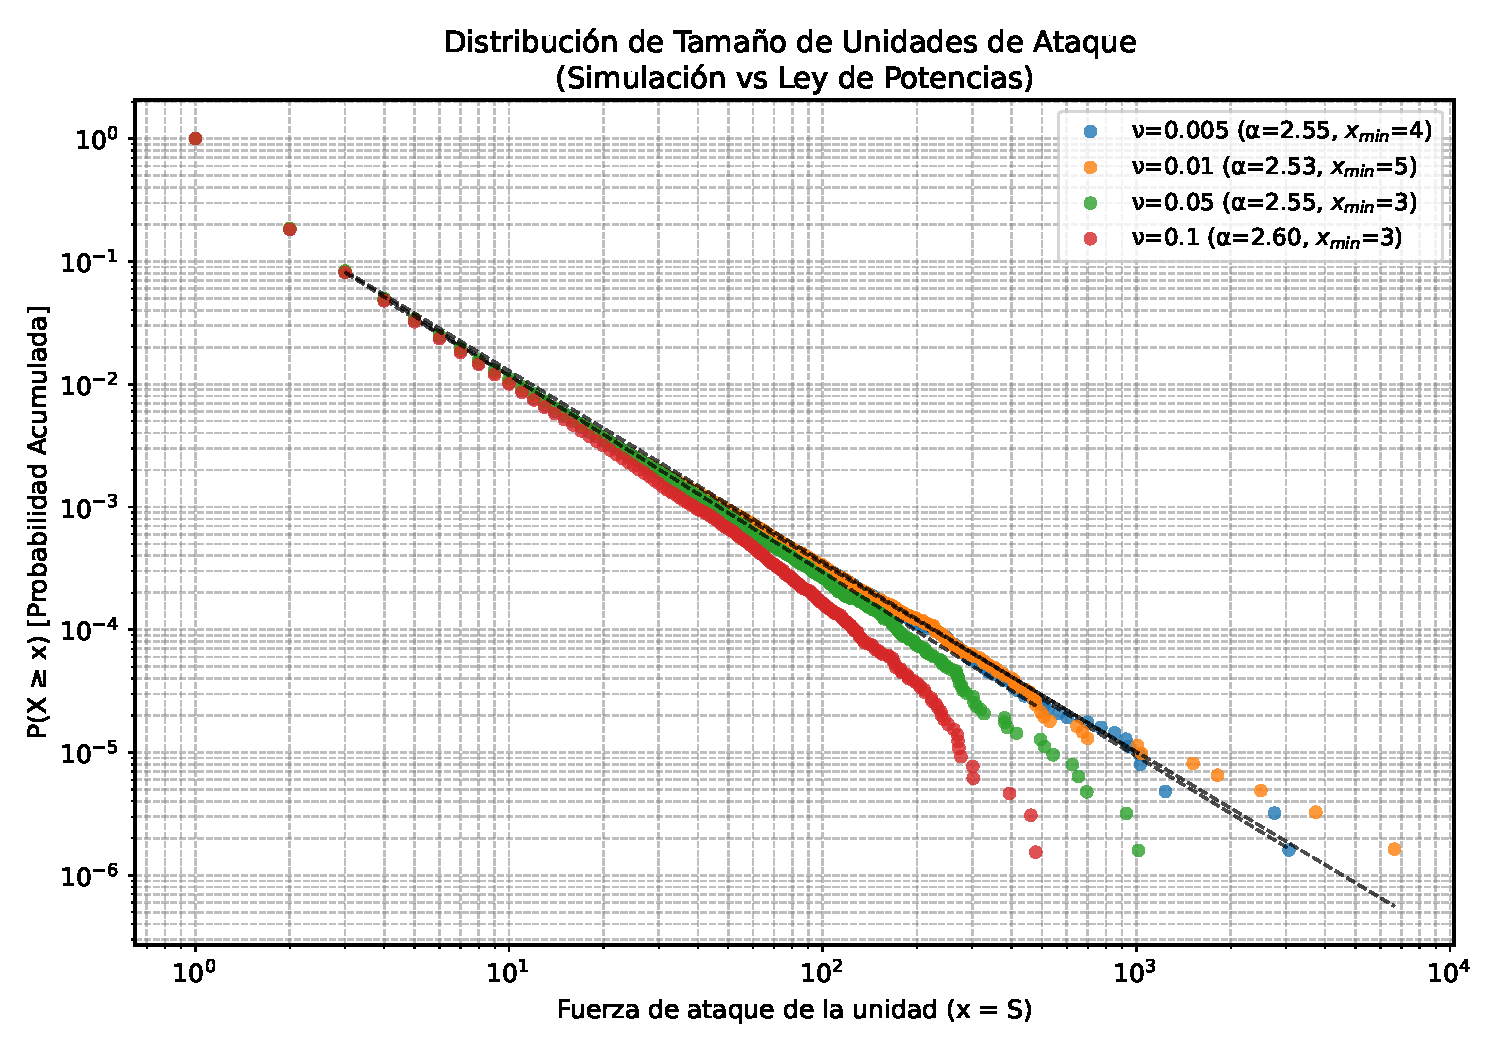
\includegraphics[width=1\linewidth]{loglog.pdf}
    \caption{Simulación de la distribución de la guerrilla.}
    \label{fig:placeholder}
\end{figure}

Este modelo muestra una tendencia a formar varias unidades de ataque con fuerza en el orden de las decenas, evitando formar unidades centralizadas; esto se puede explicar por la necesidad de distribuir la fuerza en varios sectores de la región, con la finalidad de mantener presencia en dichos sectores a la par que evitar gastar muchos recursos peleando contra las fuerzas estatales.

Otro detalle a notar es que, si la probabilidad de ataque $\nu$ es pequeña, la guerrilla tiende a formar más grupos fuertes; a medida que $\nu$ aumenta, disminuye la cantidad de unidades de ataque con alta fuerza; esto se puede atribuir a que la guerrilla necesita menos recursos para mantener su presencia y atacar, lo cual se logra explicar si el gobierno es ineficiente en combatir a estas unidades de ataque.

Finalmente, se realizó un modelado de los valores de $\alpha$ en función de la probabilidad de fragmentación $\nu$ para una partición uniforme de $100$ divisiones entre $0.005$ a $0.100$. El resultado se presenta a continuación:

\begin{figure}[h!]
    \centering
    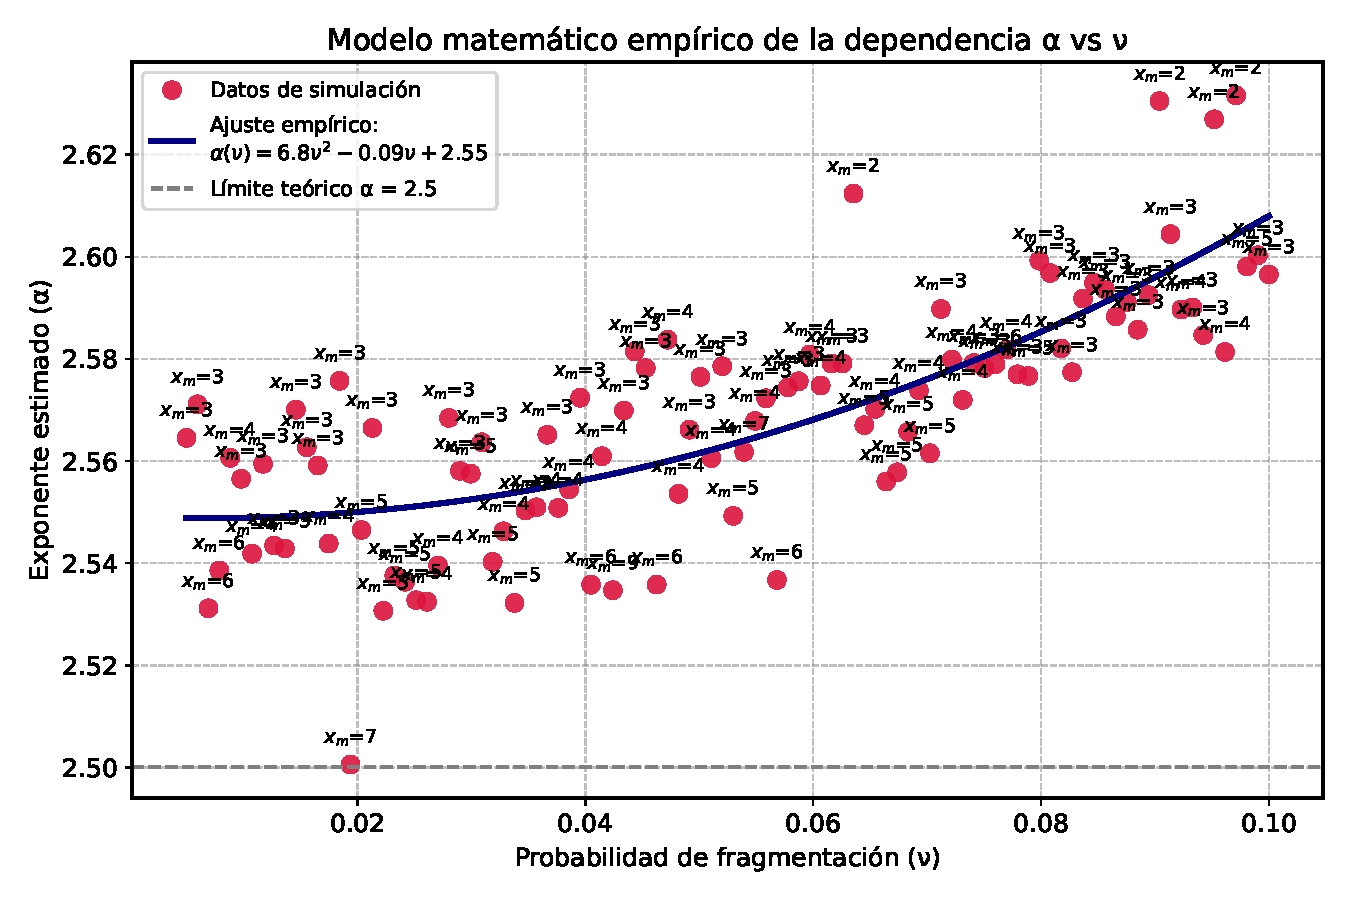
\includegraphics[width=1\linewidth]{avsv.pdf}
    \caption{Relación entre $\alpha$ y la probabilidad de fragmentación.}
    \label{fig:placeholder}
\end{figure}

\newpage

Con lo cual confirmamos el comportamiento proporcional entre $\alpha$ y $\nu$, pues evidenciamos que la guerrilla tiende a formar unidades de ataque más fuertes si su probabilidad de fragmentación (que puede estar influenciada por la fuerza del gobierno y por la superficie del territorio ocupado) es baja.

\section{Trabajo en grupo y complicaciones}

Como evidencia del trabajo en grupo, se encuentra adjunta una grabación la cual empezó desde las 7pm del 29 de Octubre de 2026 hasta y finalizó alrededor de las 3:30am del 30 de Octubre del mismo año, donde se evidencia el trabajo en grupo y también se puede ver el aporte de cada uno al código mediante el historial de commits en GitHub del repositorio \href{https://github.com/KAtoms9/CompTools-UNal}{Simulación de guerra entre guerrillas}.

La dificultad principal del proyecto fue la coordinación y manejo del tiempo de los integrantes sumado a la comprensión conceptual de los artículos proporcionados por el profesor. También fue un gran reto crear el código ya que se tuvo que aprender buena parte de comandos aleatorizadores que toman y generan valores, y pensar en cómo optimizarlo ya que los codigos iniciales podían tardar hasta 4 minutos y medio.
Otra dificultad fue usar GitHub ya que fué la primera vez de varios integrantes usándolo y bastante tiempo fue invertido en la comprensión de esta herramienta, para trabajar grupalmente fue trabajoso gracias al poco tiempo antes de la entrega del proyecto. 
A continuación se presentan dos evidencias de la reunión hecha en meet la noche anterior a la entrega del proyecto.
\begin{figure}[h!]
    \centering
    \includegraphics[width=0.8\linewidth]{Figures/Imágenes/WhatsApp Image 2026-10-29 at 11.20.55 PM.jpeg}
    \caption{Los 3 integrantes del grupo con bastantes ganas de irse a dormir}
    \label{fig:placeholder}
\end{figure}
Video con duración de 30 minutos: \href{https://drive.google.com/file/d/1SeBylkFfKLoWlEkE6QNDYBhqD1bi6baG/view?usp=sharing}{Video de 30 minutos de los integrantes del grupo }


\section{Conclusión}
El modelo presentado en Universal patterns underlying ongoing wars and terrorism refleja un comportamiento realista de las guerrillas al estudiar eventos estocásticos de reagrupación (fragmentanción y coalescencia) influenciados por un parámetro atribuido a la facilidad con la cual el grupo rebelde puede crear violencia. A mayor facilidad (probabilidad de ataque pequeña), la guerrilla tiende a conformar grupos grandes y fuertes; mientras que, con mayor dificultad (probabilidad de ataque grande), la guerrilla tiende a formar muchos grupos pequeños para garantizar su supervivencia.

\section{Bibliografía}
Johnson, N., Spagat, M., Restrepo, J., Bohórquez, J., Suárez, N., Restrepo, E., & Zarama, R. (2005). From old wars to new wars and global terrorism.
Johnson, N. F., Spagat, M., Restrepo, J. A., Becerra, O., Bohorquez, J. C., Suarez, N., Restrepo, E. M., & Zarama, R. (2006). Universal patterns underlying ongoing wars and terrorism. arXiv.

\end{document}
